\documentclass{article}

\usepackage[preprint,nonatbib]{neurips_2025}
\usepackage[numbers,sort&compress]{natbib}
\makeatletter
\renewcommand{\@noticestring}{CSL7360 Computer Vision, course project report, Team Sharanga, IIT Jodhpur, November 2026.}
\makeatother

\usepackage[utf8]{inputenc}
\usepackage[T1]{fontenc}
\renewcommand{\ttdefault}{pcr}
\renewcommand{\sfdefault}{phv}
\usepackage{hyperref}
\usepackage{url}
\usepackage{booktabs}
\usepackage{amsfonts,amsmath}
\usepackage{nicefrac}
\usepackage{microtype}
\usepackage{xcolor}
\usepackage{graphicx}
\usepackage{multirow}
\usepackage{tikz}
\usetikzlibrary{arrows.meta,positioning,fit,calc}
\hypersetup{colorlinks=true,linkcolor=blue!50!black,citecolor=blue!50!black,urlcolor=blue!50!black}



\title{What Makes Synthetic Haze Transfer to Real Haze?\\A Controlled Study of Physically Grounded Haze Synthesis}

\author{%
  Hrusikesh Nishank \\
  Department of Computer Science and Engineering\\
  Indian Institute of Technology Jodhpur \\
  \And
  Akanksha Tiwari \\
  School of Artificial Intelligence and Data Science\\
  Indian Institute of Technology Jodhpur \\
}

\begin{document}

\maketitle

\begin{abstract}
Single-image dehazing networks are trained almost entirely on synthetic hazy images, because real hazy photographs with an aligned haze-free reference are scarce. The standard recipe applies the atmospheric scattering model to a clear photograph using a relative depth map, a random scattering coefficient and a grey airlight, all in gamma-encoded sRGB. We ask which parts of this image-formation process actually matter when the trained network is applied to real haze. We build a synthesis pipeline on metric depth (Depth Pro), express haze density as a visibility in metres, draw the airlight from daylight colours, and add, one at a time, compositing in linear radiance, a camera model with sensor noise and a randomised ISP, and spatially varying extinction. Every variant shares the same clean images, depth, random numbers, network and schedule, so a difference in real-haze accuracy can be attributed to the component that changed. With DehazeFormer-T trained from scratch on 1{,}000 images, our haze improves over RESIDE's own hazy images of the same scenes by 1.0--1.4\,dB PSNR and 0.04--0.07 SSIM on O-HAZE, NH-HAZE and Dense-Haze (three seeds), and linear compositing adds up to 0.9\,dB more. The controls show where the gain comes from. A grey airlight or an uncalibrated haze density removes it entirely. When the haze density and airlight colour are calibrated on a disjoint set of real hazy photographs (RTTS) instead of the test sets' hazy inputs, most of the SSIM gain remains but the PSNR gain largely disappears, because PSNR on these benchmarks rewards matching their particular colour cast. Sensor noise and our heterogeneous-extinction model reduce accuracy. These are preliminary results from short schedules, reported with 95\% bootstrap intervals.
\end{abstract}

% =====================================================================
\section{Introduction}
\label{sec:intro}

Haze reduces contrast and shifts colour in outdoor images, and it degrades the detectors and segmenters that run on them. Removing it from a single image is ill-posed, so most current methods learn the inverse mapping from data. The difficulty is the data itself. Real hazy photographs with an aligned clear reference exist only in small benchmark sets: O-HAZE~\cite{ancuti2018ohaze}, NH-HAZE~\cite{ancuti2020nhhaze} and Dense-Haze~\cite{ancuti2019dense} together contain 155 pairs, all made with haze machines. Networks are therefore trained on synthetic pairs and evaluated, in the end, on real haze.

The most widely used synthetic set, RESIDE~\cite{li2019reside}, follows the atmospheric scattering model (ASM)~\cite{koschmieder1924,narasimhan2002vision}: a clear image $J$ is attenuated by a transmission map $t=\exp(-\beta d)$ and mixed with a constant airlight $A$. The depth $d$ comes from a monocular estimator without metric scale, $\beta$ is drawn from a fixed range, $A$ is grey, and the mixing is done directly on gamma-encoded sRGB pixel values. Each of these choices is a shortcut. Without metric depth, the same $\beta$ produces light haze in one image and heavy haze in another. A grey airlight ignores the colour of the sky that the haze scatters. Mixing in sRGB adds two light contributions after a non-linear encoding. A real camera also adds sensor noise, white-balance error, a tone curve and compression after the haze has formed.

Recent work has improved parts of this process. SynFog~\cite{xie2024synfog} path-traces fog through procedurally generated driving scenes and models the optics, sensor and ISP. HazeFlow~\cite{shin2025hazeflow} generates spatially varying haze density, and generative models learn to synthesise haze directly~\cite{wang2025hazegen}. What has not been done, to our knowledge, is the controlled comparison: keep the scenes, depth, network and training fixed, change one image-formation component at a time, and measure what each one does to accuracy on real haze. Without it, it is hard to tell whether a better synthetic dataset helps because of its physics, its haze statistics, or simply its size.

This report describes such a study, run at a small scale in the time available for the course project. Our contributions are:
\begin{enumerate}
\item A physically grounded haze synthesis pipeline on metric depth, with visibility in metres, daylight-coloured airlight, optional linear-radiance compositing, a camera and ISP model applied after the haze, and spatially varying extinction, in which all variants share their random draws.
\item A controlled evaluation of eleven synthesis variants against RESIDE's own hazy images of the same clean scenes, on four networks (two trained from scratch, two published checkpoints fine-tuned), with paired bootstrap intervals and a decision rule fixed before the runs.
\item Evidence about which components matter. A realistic distribution of haze density, which metric depth and visibility make controllable, improves structural accuracy (SSIM) even when it is calibrated on a different real dataset. Matching the airlight colour of the target data accounts for most of the PSNR gain. Linear compositing helps when training from scratch, and sensor noise and our heterogeneous-extinction model hurt.
\end{enumerate}

\paragraph{Relation to our project proposal.} Our proposal set three objectives: a forward-rendered paired dataset from 3D reconstructions of real scenes, a controlled ablation of the synthesis components with scenes and network held fixed, and a wavelength-dependent model of South Asian pollution haze. The proposal named the controlled ablation as the scientific core and the fallback if reconstruction proved too slow, and that is what this report carries out, on monocular metric depth instead of 3D reconstructions. The proposal's central claim, that removing the camera and ISP stage costs more accuracy than removing haze heterogeneity, is tested in Section~\ref{sec:components}, and is not supported in the form we stated it. The other two objectives remain future work (Section~\ref{sec:conclusion}).

\paragraph{Code.} The code, the per-run results and the scripts that produce every number and table in this report are in the GitHub repository \texttt{hrusikesh-nishank/CV-Dehazing-Study}.

% =====================================================================
\section{Literature Review}
\label{sec:related}

\paragraph{Haze imaging models and priors.} Koschmieder's law~\cite{koschmieder1924} describes the apparent luminance of an object seen through a homogeneous scattering medium, and Narasimhan and Nayar~\cite{narasimhan2002vision} formalised it for computer vision as the ASM, $I = J\,t + A(1-t)$ with $t=\exp(-\beta d)$. The meteorological optical range links $\beta$ to visibility: with a 5\% contrast threshold, $\beta = 2.996/V$~\cite{wmo2018guide}. Some synthesis work instead uses a 2\% threshold ($\beta=3.912/V$), which gives about 30\% more extinction for the same stated visibility. We use the 5\% convention throughout. The dark channel prior (DCP)~\cite{he2011dcp} estimates $t$ from the observation that, in haze-free outdoor patches, at least one colour channel has a very dark pixel. It needs no training data and remains a strong baseline on dense haze.

\paragraph{Synthetic training data.} RESIDE~\cite{li2019reside} applies the ASM to indoor and outdoor photographs using estimated depth, random $\beta$ and grey $A$, and its outdoor training set (OTS) is the most common source of pre-trained dehazing weights. Foggy Cityscapes~\cite{sakaridis2018foggy} uses stereo depth on driving scenes and specifies fog by visibility. RIDCP~\cite{wu2023ridcp} adds further degradations to its synthetic pairs, including a colour-shifted airlight and JPEG compression. SynFog~\cite{xie2024synfog} renders spectral radiance by volumetric path tracing in procedural scenes and passes it through an optics, sensor and ISP simulation. Its ablation is the closest precedent to ours: applying the plain ASM to its own clear images, with exact depth, transferred clearly worse to real fog than the full rendering pipeline. HazeFlow~\cite{shin2025hazeflow} reformulates the ASM as an ODE and generates non-homogeneous haze with Markov-chain Brownian motion. Its training data include real unpaired hazy images, RTTS among them. Generative approaches~\cite{wang2025hazegen} learn the haze appearance from data. These works each change several components of image formation at once and evaluate the resulting dataset or method as a whole.

\paragraph{Dehazing networks and benchmarks.} We use three recent architectures with public code and weights. DehazeFormer~\cite{song2023dehazeformer} adapts the Swin Transformer to dehazing, gUNet~\cite{song2022gunet} is a gated U-Net that reaches similar accuracy with convolutions only, and DEA-Net~\cite{chen2024deanet} combines detail-enhanced convolution with content-guided attention. On synthetic test sets their PSNR is above 30\,dB; on the real O-HAZE, NH-HAZE and Dense-Haze pairs, models trained on RESIDE reach about 12--17\,dB. RTTS~\cite{li2019reside} provides 4{,}322 real hazy images with object annotations but no clear reference, and is used for detection-based and no-reference evaluation.

\paragraph{Camera modelling.} Brooks et al.~\cite{brooks2019unprocessing} showed that sRGB images can be ``unprocessed'' into plausible raw sensor data by inverting the tone curve, gamma, colour correction and white balance, and that adding noise in that space improves learned denoising. We use their camera model to form haze in linear radiance and to add noise and ISP effects after the haze, as a real camera would.

\paragraph{Gap.} No published study holds the scenes, depth and network fixed and changes one haze-formation component at a time, measuring the effect on real haze. This is the gap the present study addresses.

% =====================================================================
\section{Problem Statement}
\label{sec:problem}

Let $\{J_i\}$ be clear outdoor images with metric depth maps $\{d_i\}$. A synthesis procedure $S_\phi$ turns a clear image into a hazy image and a training target, $(I_i, T_i) = S_\phi(J_i, d_i, \xi_i)$, where $\xi_i$ are random draws (visibility, airlight, camera parameters, crops) and $\phi$ is the set of image-formation components switched on. A dehazing network $f_\theta$ is trained on these pairs and then applied, without adaptation, to real hazy images $\{(H_k, G_k)\}$ with reference images $G_k$. We measure zero-shot accuracy by PSNR and SSIM on the real pairs, and by detection and no-reference quality on RTTS.

The question is how much each component in $\phi$ changes real-haze accuracy when everything else is held fixed: the clear images, depth maps, random draws $\xi_i$, network, initialisation, and training schedule. Before running anything we fixed the following rules:
\begin{itemize}
\item A difference is reported as an effect only if its 95\% paired bootstrap interval over test images excludes zero and, where several seeds exist, it exceeds twice the seed-to-seed standard deviation. Differences below 0.3\,dB on O-HAZE (45 images) are treated as noise.
\item Our initial hypothesis was that the camera model would matter more than spatial heterogeneity of the extinction. NH-HAZE, whose haze is non-homogeneous by design, was declared in advance as the set where heterogeneity could matter most.
\end{itemize}

% =====================================================================
\section{Proposed Method}
\label{sec:method}

Figure~\ref{fig:pipeline} summarises the pipeline. Each stage is a switch that defines one variant (an ``arm'') of the training data.

\begin{figure}[t]
\centering
\resizebox{\linewidth}{!}{%
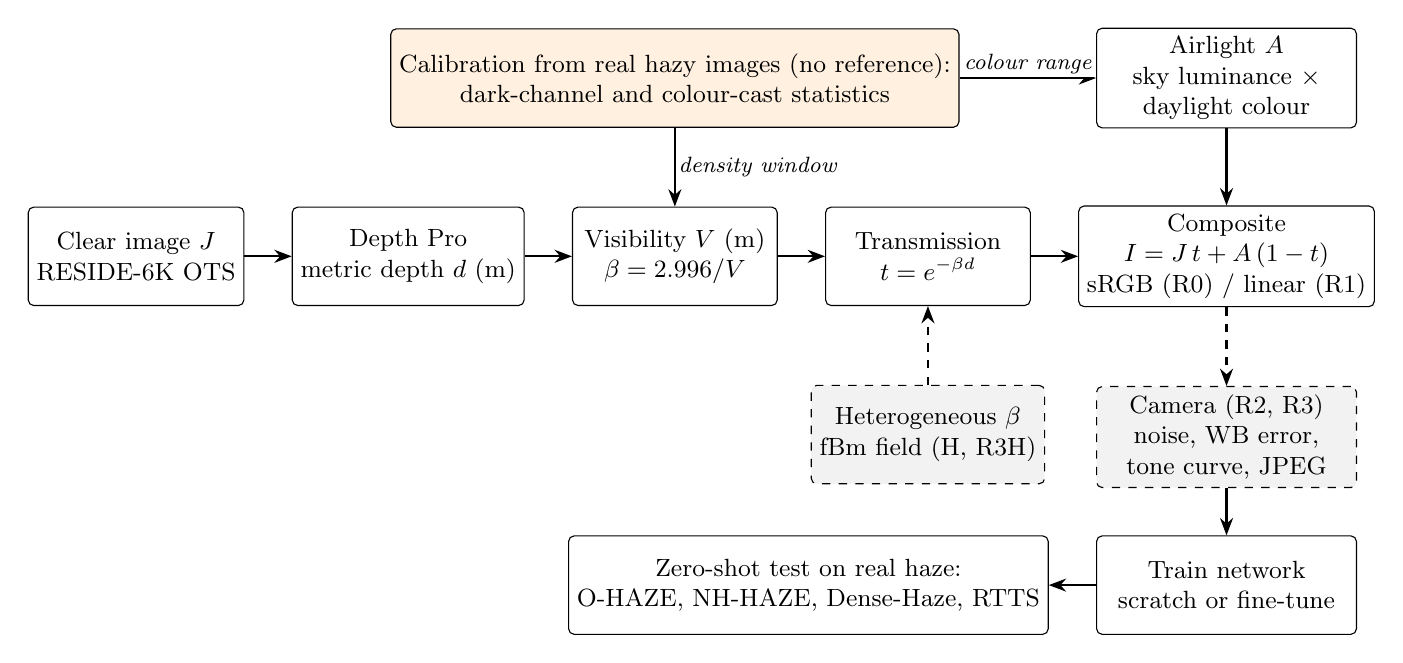
\begin{tikzpicture}[
  box/.style={draw, rounded corners=2pt, align=center, font=\small, minimum height=1.25cm, minimum width=2.6cm, inner sep=3pt, fill=white},
  opt/.style={box, dashed, fill=gray!10},
  cal/.style={box, fill=orange!12},
  lab/.style={font=\footnotesize\itshape, fill=white, inner sep=1pt},
  arr/.style={-{Stealth[length=2.2mm]}, thick}]
% row 2: the synthesis chain
\node[box] (J) {Clear image $J$\\RESIDE-6K OTS};
\node[box, right=0.6cm of J] (D) {Depth Pro\\metric depth $d$ (m)};
\node[box, right=0.6cm of D] (V) {Visibility $V$ (m)\\$\beta = 2.996/V$};
\node[box, right=0.6cm of V] (T) {Transmission\\$t = e^{-\beta d}$};
\node[box, right=0.6cm of T, minimum width=3.3cm] (C) {Composite\\$I = J\,t + A\,(1-t)$\\sRGB (R0) / linear (R1)};
% row 1: calibration and airlight
\node[cal, above=1.0cm of V, minimum width=5.6cm] (cal) {Calibration from real hazy images (no reference):\\dark-channel and colour-cast statistics};
\node[box, minimum width=3.3cm] (A) at (C |- cal) {Airlight $A$\\sky luminance $\times$\\daylight colour};
% row 3: optional modules
\node[opt, below=1.0cm of T] (H) {Heterogeneous $\beta$\\fBm field (H, R3H)};
\node[opt, below=1.0cm of C, minimum width=3.3cm] (cam) {Camera (R2, R3)\\noise, WB error,\\tone curve, JPEG};
% row 4: training and testing
\node[box, below=0.6cm of cam, minimum width=3.3cm] (N) {Train network\\scratch or fine-tune};
\node[box, left=0.6cm of N, minimum width=5.6cm] (E) {Zero-shot test on real haze:\\O-HAZE, NH-HAZE, Dense-Haze, RTTS};
% arrows
\draw[arr] (J) -- (D);
\draw[arr] (D) -- (V);
\draw[arr] (V) -- (T);
\draw[arr] (T) -- (C);
\draw[arr] (cal) -- node[lab, right] {density window} (V);
\draw[arr] (cal) -- node[lab, above] {colour range} (A);
\draw[arr] (A) -- (C);
\draw[arr, dashed] (H) -- (T);
\draw[arr, dashed] (C) -- (cam);
\draw[arr] (cam) -- (N);
\draw[arr] (N) -- (E);
\end{tikzpicture}}
\caption{Synthesis pipeline. Solid boxes are used by every arm; dashed boxes are switched on only in some arms (the camera for R2, R3 and R3N; the heterogeneous field for H and R3H). The orange box is the calibration step: the haze density window and the airlight colour range are set from statistics of real hazy images, without their reference images. All arms share the same depth maps and random draws.}
\label{fig:pipeline}
\end{figure}

\subsection{Metric depth and visibility}
We take the 3{,}000 clear outdoor images of RESIDE-6K (400$\times$400 pixels) and estimate metric depth with Depth Pro~\cite{bochkovskii2025depthpro}, which predicts absolute scale without camera intrinsics. Sky pixels receive large depths; the median scene depth ranges from about 3\,m for close-ups to over 100\,m for city views (5th--95th percentile). Haze density is set by a visibility $V$ in metres through $\beta = 2.996/V$. For each image we draw eight $(V, A)$ pairs once and store them, so every arm sees exactly the same haze geometry. $V$ is drawn log-uniformly between 10\,m and 5\,km and redrawn until the image's mean transmission falls inside a window $[t_{lo}, t_{hi}]$. Without this window, a close-up scene almost never receives visible haze and a city view at 50\,m visibility becomes uniformly white.

\subsection{Airlight}
The airlight luminance is taken from the brightest 10\% of pixels in the far region of the image (clipped to $[0.55, 0.98]$, with a random fallback when no sky is present). Its colour is a CIE daylight chromaticity at a correlated colour temperature drawn uniformly in mired, expressed relative to D65 at equal luminance. This gives a slightly bluish airlight for high temperatures and a warmer one for low temperatures. The grey-airlight arm N0 keeps the luminance and drops the colour.

\paragraph{Calibration from real hazy images.} The density window and the colour-temperature range are the two places where we use statistics of real haze. We measured, on the hazy images only, the mean dark-channel value (a proxy for haze density) and the blue-minus-red cast of the brightest region. Across O-HAZE, NH-HAZE, Dense-Haze and RTTS the 5th--95th percentile of the dark-channel mean spans 0.24--0.73, and the cast spans $-0.12$ to $+0.17$. A transmission window of $[0.10, 0.85]$ and daylight between 5{,}500\,K and 9{,}500\,K reproduce these ranges. No reference image is used, but the test sets' hazy inputs are. We therefore also train with an uncalibrated variant (R0\textsubscript{unc}: $V\in[50\,\text{m}, 5\,\text{km}]$ log-uniform, no window, 5{,}000--10{,}000\,K) and with a variant calibrated only on RTTS (R0\textsubscript{rtts}, R1\textsubscript{rtts}: window $[0.17, 0.70]$, 5{,}600--7{,}500\,K), whose images are never used in the PSNR evaluation.

\subsection{Compositing in sRGB and in linear radiance}
The baseline arm R0 applies the ASM directly to sRGB values, as RESIDE does. Arm R1 first converts $J$ and $A$ to linear radiance by inverting a global tone curve and a 2.2 gamma (following Brooks et al.~\cite{brooks2019unprocessing}), composites there, and converts back with the same curve. The difference is largest in dark regions, where sRGB mixing adds too much airlight. For a dark pixel ($J=0.1$) with $t=0.5$ and $A=0.9$, sRGB mixing gives 0.50, while linear mixing gives 0.65 after re-encoding.

\subsection{Camera model}
Arms R2 and R3 pass the linear composite through a camera. We follow Brooks et al.~\cite{brooks2019unprocessing}: a random colour-correction matrix and white-balance gains map linear sRGB into camera space, where Poisson--Gaussian noise is added \emph{after} the haze. Shot-noise variance is drawn log-uniformly in $[2\times10^{-5}, 8\times10^{-4}]$, a daylight range, and read noise follows Brooks' log-linear relation. The ISP then applies white balance with a 3\% random error, the colour matrix, gamma and a randomly weighted tone curve. Finally, 70\% of images are JPEG-compressed at quality 60--95. R2 adds only the noise to R1, R3 adds the full camera, and R3N is R3 without noise. For arms with a randomised tone curve, the training target is the clear image passed through the same tone curve, so the network is not asked to undo a random global contrast change it cannot observe. We do not simulate a Bayer mosaic by default: the 400-pixel images are far below sensor resolution, where demosaicing blur is negligible.

\subsection{Heterogeneous extinction and other arms}
Arms H and R3H multiply $\beta$ by $\exp(0.4\,n)$, where $n$ is a unit-variance fractal (fBm) noise field, and renormalise so that the mean extinction is unchanged. N0 uses a grey airlight. B0 uses RESIDE's own hazy images of the same 1{,}000 clear images, so it differs from R0 in depth source, haze-density distribution, airlight and its synthesis code.

\subsection{Controlled design}
All random quantities (crop position, flip, $(V,A)$ draw, camera parameters, ISP parameters, JPEG quality, noise, heterogeneity field) come from separate random streams seeded by (seed, image index, epoch). Two arms that share a component therefore share its random numbers. For example, R3 and R3H use the same cameras, and R0 and R1 the same visibilities. A difference between two arms can then only come from the component that differs.

\begin{figure}[t]
\centering
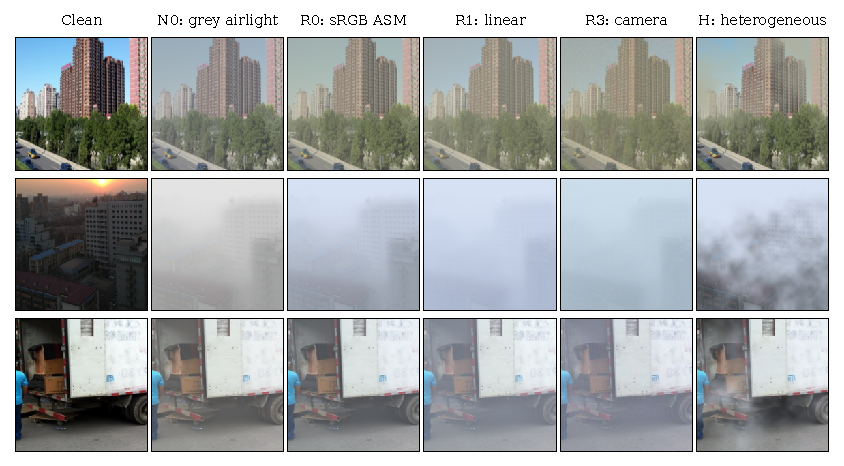
\includegraphics[width=\linewidth]{figs/synthesis.pdf}
\caption{The same three clear images under several arms, with identical visibility and airlight draws. N0 uses a grey airlight; R1 composites in linear radiance (note the lighter dark regions); R3 adds the camera (noise, white-balance error, tone curve, JPEG); H adds a heterogeneous extinction field.}
\label{fig:synthesis}
\end{figure}

% =====================================================================
\section{Experiments and Results}
\label{sec:experiments}

\subsection{Setup}
\paragraph{Training.} All arms use the first 1{,}000 clear images of RESIDE-6K OTS (sorted by name) and their stored $(V,A)$ draws. DehazeFormer-T and gUNet-T are trained from scratch with the official DehazeFormer recipe: AdamW, $L_1$ loss, learning rate $4\times10^{-4}$ with a linear warm-up and cosine decay to 1\%, batch 16, random 256$\times$256 crops with horizontal flips, and mixed precision. Each arm runs 3{,}500 iterations for DehazeFormer-T (about 56 epochs) and 8{,}400 for gUNet-T. The published DehazeFormer-B and DEA-Net checkpoints (trained on RESIDE-OTS) are fine-tuned for 2{,}100 and 4{,}600 iterations at learning rate $10^{-4}$ (batch 4 and 8). Their B0 rows fine-tune on RESIDE's hazy images for the same number of iterations, which separates the effect of our data from the effect of extra training. All runs used one RTX 5060 Ti (16\,GB); one from-scratch run takes about 22 minutes. The schedules were set so that the whole study fits into a few nights of GPU time, which is short compared with the original training of the published models.

\paragraph{Evaluation.} Paired test sets are resized so that the long side is 1{,}024 pixels, the network runs on the full image (tiled only when memory runs out), and outputs are quantised to 8 bits. PSNR is computed on RGB in $[0,1]$ and SSIM with a Gaussian window ($\sigma=1.5$). For RTTS we use a fixed subset of 500 images: detection mAP$_{50}$ with a COCO-trained YOLOv8m~\cite{jocher2023yolov8} on the five RTTS classes, following the VOC protocol and ignoring objects marked difficult, and NIQE~\cite{mittal2013niqe}, BRISQUE~\cite{mittal2012brisque}, MUSIQ~\cite{ke2021musiq} and CLIP-IQA~\cite{wang2023clipiqa} on 100 of them. All rows, including the published models, are evaluated by the same code. Intervals are 95\% paired bootstrap intervals over test images (10{,}000 resamples)~\cite{efron1993bootstrap}, computed on seed-averaged per-image scores.

\paragraph{Is the synthetic haze in the range of real haze?} Before training, we compared the dark-channel mean of 300 synthetic crops with real RTTS crops. The 5th/50th/95th percentiles are 0.25/0.48/0.76 for R0 and 0.17/0.47/0.75 for RTTS, and the blue-minus-red cast overlaps as well. Kernel inception distance~\cite{binkowski2018kid} to RTTS is lowest for R1 ($22.5\times10^{-3}$) and highest for the heterogeneous arms (31.0 and $35.7\times10^{-3}$), with a standard error of about $3.5\times10^{-3}$.

\subsection{Comparison with published models}
Table~\ref{tab:main} places the published checkpoints and our trained models under one protocol. The published models, trained for far longer on the full RESIDE-OTS set, reach 16.1--16.7\,dB on O-HAZE; DCP reaches 16.1\,dB and is the best method on Dense-Haze (12.54\,dB). DehazeFormer-T trained for 22 minutes on 1{,}000 images of our haze (R1, three seeds) reaches 18.17\,dB on O-HAZE and 13.44\,dB on NH-HAZE, above every published checkpoint, while the same network trained on RESIDE's hazy versions of the same images (B0) reaches 15.88\,dB. Fine-tuning the published DehazeFormer-B and DEA-Net on our data raises their O-HAZE PSNR to 18.61 and 18.69\,dB; fine-tuning them on RESIDE's images for the same number of steps leaves them near their starting point (16.25 and 16.85\,dB). The improvement therefore comes from the data, not from the additional training. These rows use the calibration on the test sets' hazy inputs; Section~\ref{sec:calib} shows how much of the gain depends on it.

\begin{table}[t]
\caption{Zero-shot results on real paired haze. All rows are evaluated with the same code at a long side of 1{,}024 pixels; no numbers are copied from papers. The upper block uses the published weights. $^{\times n}$: mean over $n$ seeds. Best value per column in bold.}
\label{tab:main}
\centering
\small
\resizebox{\linewidth}{!}{\begin{tabular}{llcccccc}
\toprule
Method & Training data & \multicolumn{2}{c}{O-HAZE} & \multicolumn{2}{c}{NH-HAZE} & \multicolumn{2}{c}{Dense-Haze} \\
\cmidrule(lr){3-4}\cmidrule(lr){5-6}\cmidrule(lr){7-8}
 & & PSNR & SSIM & PSNR & SSIM & PSNR & SSIM \\
\midrule
Hazy input & -- & 13.78 & 0.619 & 11.48 & 0.451 & 9.61 & 0.404 \\
DCP~\cite{he2011dcp} & none (prior) & 16.07 & 0.677 & 12.31 & 0.473 & \textbf{12.54} & 0.425 \\
DehazeFormer-T~\cite{song2023dehazeformer} & RESIDE-OTS & 16.08 & 0.681 & 12.17 & 0.488 & 11.24 & 0.436 \\
DehazeFormer-B~\cite{song2023dehazeformer} & RESIDE-OTS & 16.20 & 0.683 & 12.18 & 0.486 & 11.23 & 0.435 \\
DEA-Net~\cite{chen2024deanet} & RESIDE-OTS & 16.67 & 0.705 & 12.37 & 0.506 & 11.57 & 0.443 \\
\midrule \multicolumn{8}{l}{\emph{Trained here (1{,}000 clean images, short schedule)}} \\
DehazeFormer-T, scratch$^{\times3}$ & B0 (RESIDE pairs) & 15.88 & 0.673 & 12.08 & 0.483 & 10.79 & 0.422 \\
DehazeFormer-T, scratch$^{\times3}$ & R0 (ours, sRGB) & 17.25 & 0.743 & 13.10 & 0.556 & 12.12 & 0.459 \\
DehazeFormer-T, scratch$^{\times3}$ & R1 (ours, linear) & 18.17 & 0.757 & 13.44 & 0.573 & 12.02 & 0.458 \\
DehazeFormer-T, scratch & R1, RTTS-calibrated & 15.83 & 0.733 & 12.24 & 0.557 & 11.40 & 0.440 \\
gUNet-T, scratch & B0 (RESIDE pairs) & 16.38 & 0.692 & 12.17 & 0.493 & 10.81 & 0.418 \\
gUNet-T, scratch & R1 (ours, linear) & 18.45 & \textbf{0.775} & 13.30 & \textbf{0.584} & 11.58 & 0.471 \\
DehazeFormer-B, fine-tuned & B0 (RESIDE pairs) & 16.25 & 0.680 & 12.22 & 0.484 & 11.21 & 0.433 \\
DehazeFormer-B, fine-tuned & R3 (ours, camera) & 18.61 & 0.765 & \textbf{13.45} & 0.562 & 12.18 & \textbf{0.495} \\
DEA-Net, fine-tuned & B0 (RESIDE pairs) & 16.85 & 0.698 & 12.44 & 0.498 & 11.48 & 0.438 \\
DEA-Net, fine-tuned & R0 (ours, sRGB) & \textbf{18.69} & 0.756 & 13.11 & 0.547 & 11.79 & 0.460 \\
\bottomrule
\end{tabular}}
\end{table}

\subsection{Which image-formation components matter}
\label{sec:components}
Table~\ref{tab:steps} and Figure~\ref{fig:effects} isolate each component for DehazeFormer-T trained from scratch; Table~\ref{tab:arms} in the appendix lists the absolute numbers.

\paragraph{Haze density and airlight colour.} Our sRGB arm R0 is 1.38, 1.02 and 1.33\,dB better than RESIDE's hazy images (B0) on the three sets (three seeds each), and all three intervals exclude zero. Two controls show what this gain needs. Removing the airlight colour (N0) makes the result \emph{worse} than B0 by 0.5--1.0\,dB, and the sky-coloured airlight alone accounts for 1.5--2.4\,dB (R0 $-$ N0). Removing the density window (R0\textsubscript{unc}) brings the result back to the level of B0, within 0.3\,dB on all three sets. Metric depth and visibility in metres make haze density and colour controllable, but on their own (N0, R0\textsubscript{unc}) they do not help. The next subsection asks how much of the gain depends on calibrating these two quantities on the test sets.

\paragraph{Compositing in linear radiance.} R1 improves over R0 by 0.91 and 0.34\,dB on O-HAZE and NH-HAZE, with both intervals above zero over three seeds, and is within noise on Dense-Haze ($-0.10$\,dB). R1 is the best arm overall and beats B0 by 2.29, 1.36 and 1.23\,dB.

\paragraph{Camera model.} Adding sensor noise after the haze (R2) costs 0.81, 0.34 and 0.49\,dB relative to R1, the largest negative effect apart from heterogeneity. The randomised ISP and JPEG recover part of this (R3 $-$ R2 $\approx$ +0.3\,dB on two sets). Without noise, the ISP and JPEG (R3N) are within noise of R1 on all three sets. In this setting, then, the camera model as a whole does not help, and its noise component hurts. One likely reason is resolution. The noise is added at the 400-pixel training resolution with daylight sensor statistics, while the test images are downsampled from multi-megapixel photographs to a 1{,}024-pixel side, which averages most sensor noise away. A network trained to remove noise that the test images do not have smooths away real detail. We have not yet tested this explanation.

\paragraph{Heterogeneous extinction.} Adding the fBm extinction field reduces PSNR by 1.8, 0.6 and 2.4\,dB (H $-$ R0) and by a similar amount in the camera arm (R3H $-$ R3), including on NH-HAZE, the set declared in advance as most likely to benefit. Our field produces smoke-like blobs (Figure~\ref{fig:synthesis}) that resemble neither the haze-machine plumes of NH-HAZE nor natural haze, and the KID check above already ranked these arms furthest from real haze. In our pre-registered comparison, adding the camera to the heterogeneous arm (R3H $-$ H) changes PSNR by $-0.01$, $+0.41$ and $-0.13$\,dB, while adding heterogeneity to the camera arm (R3H $-$ R3) changes it by $-2.18$, $-0.18$ and $-2.23$\,dB. Heterogeneity therefore has the larger effect, but in the harmful direction, so the comparison does not support the hypothesis in the form we stated it.

\begin{table}[t]
\caption{Effect of each component for DehazeFormer-T trained from scratch: PSNR difference (dB) between two arms with 95\% paired bootstrap interval. Bold: the interval excludes zero and $|\Delta| \ge 0.3$\,dB. Seeds: number of seeds for $A$/$B$.}
\label{tab:steps}
\centering
\small
\resizebox{\linewidth}{!}{\begin{tabular}{lcccc}
\toprule
Comparison ($A - B$) & O-HAZE & NH-HAZE & Dense-Haze & Seeds \\
\midrule
Our haze (sRGB ASM) vs.\ RESIDE haze (R0 $-$ B0) & \textbf{+1.38} {\scriptsize[+0.93, +1.83]} & \textbf{+1.02} {\scriptsize[+0.75, +1.31]} & \textbf{+1.33} {\scriptsize[+0.89, +1.78]} & 3/3 \\
\quad same with grey airlight (N0 $-$ B0) & \textbf{-1.00} {\scriptsize[-1.25, -0.75]} & \textbf{-0.46} {\scriptsize[-0.60, -0.32]} & \textbf{-0.71} {\scriptsize[-1.10, -0.33]} & 1/3 \\
\quad same without density calibration (R0\_uncal $-$ B0) & -0.16 {\scriptsize[-0.50, +0.19]} & +0.08 {\scriptsize[-0.05, +0.22]} & -0.28 {\scriptsize[-0.56, -0.02]} & 1/3 \\
\quad same, calibrated on RTTS only (R0\_rtts $-$ B0) & -0.08 {\scriptsize[-0.44, +0.28]} & +0.19 {\scriptsize[-0.02, +0.41]} & \textbf{+0.45} {\scriptsize[+0.02, +0.89]} & 1/3 \\
\addlinespace
Sky-coloured vs.\ grey airlight (R0 $-$ N0) & \textbf{+2.38} {\scriptsize[+1.92, +2.87]} & \textbf{+1.48} {\scriptsize[+1.18, +1.81]} & \textbf{+2.04} {\scriptsize[+1.50, +2.63]} & 3/1 \\
\addlinespace
+ linear-radiance compositing (R1 $-$ R0) & \textbf{+0.91} {\scriptsize[+0.65, +1.17]} & \textbf{+0.34} {\scriptsize[+0.22, +0.46]} & -0.10 {\scriptsize[-0.30, +0.08]} & 3/3 \\
+ sensor noise after haze (R2 $-$ R1) & \textbf{-0.81} {\scriptsize[-1.01, -0.61]} & \textbf{-0.34} {\scriptsize[-0.48, -0.21]} & \textbf{-0.49} {\scriptsize[-0.84, -0.17]} & 1/3 \\
+ randomised ISP and JPEG (R3 $-$ R2) & +0.29 {\scriptsize[+0.06, +0.52]} & +0.01 {\scriptsize[-0.08, +0.10]} & +0.29 {\scriptsize[+0.14, +0.44]} & 2/1 \\
ISP and JPEG without noise (R3N $-$ R1) & -0.01 {\scriptsize[-0.22, +0.20]} & -0.08 {\scriptsize[-0.16, -0.01]} & +0.01 {\scriptsize[-0.14, +0.17]} & 1/3 \\
\addlinespace
+ heterogeneous extinction (sRGB) (H $-$ R0) & \textbf{-1.79} {\scriptsize[-2.32, -1.29]} & \textbf{-0.58} {\scriptsize[-0.86, -0.33]} & \textbf{-2.41} {\scriptsize[-2.86, -1.94]} & 1/3 \\
+ heterogeneous extinction (camera) (R3H $-$ R3) & \textbf{-2.18} {\scriptsize[-2.78, -1.62]} & -0.18 {\scriptsize[-0.43, +0.06]} & \textbf{-2.23} {\scriptsize[-2.59, -1.87]} & 1/2 \\
\addlinespace
Best variant (R1) vs.\ RESIDE haze (R1 $-$ B0) & \textbf{+2.29} {\scriptsize[+1.72, +2.87]} & \textbf{+1.36} {\scriptsize[+1.10, +1.63]} & \textbf{+1.23} {\scriptsize[+0.82, +1.64]} & 3/3 \\
\quad R1 calibrated on RTTS only (R1\_rtts $-$ B0) & -0.05 {\scriptsize[-0.42, +0.34]} & +0.16 {\scriptsize[-0.08, +0.44]} & \textbf{+0.61} {\scriptsize[+0.15, +1.09]} & 1/3 \\
\bottomrule
\end{tabular}}
\end{table}

\begin{figure}[t]
\centering
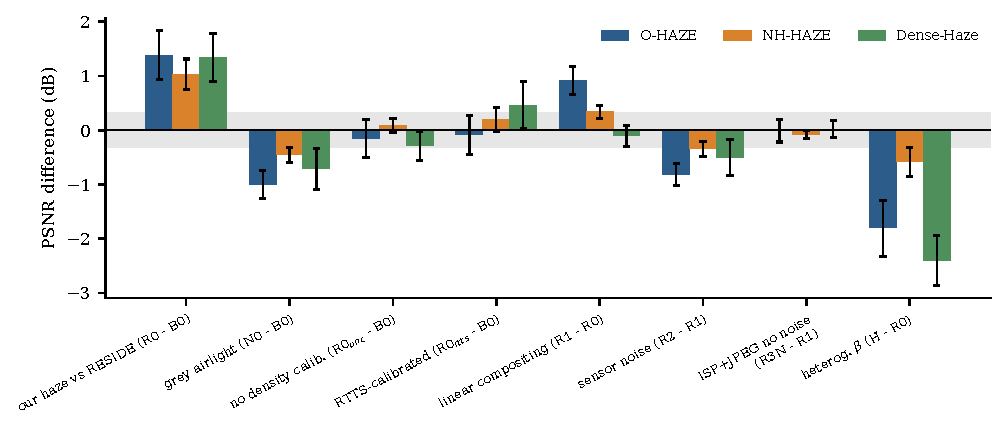
\includegraphics[width=\linewidth]{figs/effects.pdf}
\caption{Effect sizes from Table~\ref{tab:steps} (DehazeFormer-T). The grey band marks $\pm0.3$\,dB, our noise threshold. Error bars are 95\% bootstrap intervals over test images.}
\label{fig:effects}
\end{figure}

\subsection{How much of the gain depends on calibration?}
\label{sec:calib}
Our density window and colour range were set from the hazy inputs of the evaluation sets (and RTTS). No reference image was used, but a reader may still ask whether the gain is a form of tuning to the test data. To test this we recalibrated both quantities on RTTS alone, a separate collection of real hazy photographs that we never use for PSNR or SSIM, and retrained. Table~\ref{tab:calib} reports PSNR and SSIM differences against B0.

The two metrics react differently. With RTTS calibration, SSIM still improves over B0 on all three sets (+0.057, +0.067 and +0.021 for R0\textsubscript{rtts}), which is about 80\% of the SSIM gain obtained with test-set calibration. PSNR, however, no longer improves on O-HAZE ($-0.08$\,dB) or NH-HAZE (+0.19\,dB, within noise), and improves only on Dense-Haze (+0.45\,dB). The uncalibrated arm improves neither. Comparing the two calibrations directly (R0 $-$ R0\textsubscript{rtts}) gives large PSNR differences (+0.8 to +1.5\,dB) but small SSIM differences (+0.006 to +0.016). The test-set calibration therefore mainly buys colour and brightness agreement, which PSNR rewards heavily. This is plausible from the data: the haze-machine sets have a bluish cast (median blue-minus-red +0.05 to +0.08), whereas RTTS haze is close to neutral, so the RTTS calibration (5{,}600--7{,}500\,K) draws none of the bluish airlights that these test sets contain. The structural improvement comes from a realistic spread of haze density, and it transfers across datasets. For gUNet-T the RTTS-calibrated R1 still beats B0 in PSNR on O-HAZE and NH-HAZE (+0.58 and +0.63\,dB) and in SSIM on all three sets. Under RTTS calibration, linear compositing no longer changes PSNR for DehazeFormer-T (R1\textsubscript{rtts} $-$ R0\textsubscript{rtts}: +0.04, $-0.03$ and +0.16\,dB, all within noise).

In practical terms, the synthesis should be calibrated on unlabelled hazy images from the target domain, which requires no reference images. With such data, the gain is large. Without it, metric-depth haze with a realistic density distribution still improves structure over RESIDE, but PSNR gains on a new domain should not be expected.

\begin{table}[t]
\caption{Calibration controls: difference to B0 (or between calibrations) in PSNR and SSIM. Bold: 95\% bootstrap interval excludes zero (and $|\Delta|\ge0.3$\,dB for PSNR). DehazeFormer-T R0 and B0 use three seeds, all other arms one.}
\label{tab:calib}
\centering
\small
\resizebox{\linewidth}{!}{\begin{tabular}{llcccccc}
\toprule
Network & Comparison & \multicolumn{3}{c}{$\Delta$PSNR (dB)} & \multicolumn{3}{c}{$\Delta$SSIM} \\
\cmidrule(lr){3-5}\cmidrule(lr){6-8}
 & & O & NH & Dense & O & NH & Dense \\
\midrule
DehazeFormer-T & R0 $-$ B0 (calibrated on test-set hazy inputs) & \textbf{+1.38} & \textbf{+1.02} & \textbf{+1.33} & \textbf{+0.070} & \textbf{+0.073} & \textbf{+0.037} \\
DehazeFormer-T & R0\_uncal $-$ B0 (not calibrated) & -0.16 & +0.08 & -0.28 & -0.003 & \textbf{+0.004} & +0.000 \\
DehazeFormer-T & R0\_rtts $-$ B0 (calibrated on RTTS only) & -0.08 & +0.19 & \textbf{+0.45} & \textbf{+0.057} & \textbf{+0.067} & \textbf{+0.021} \\
DehazeFormer-T & R1\_rtts $-$ B0 (R1, calibrated on RTTS only) & -0.05 & +0.16 & \textbf{+0.61} & \textbf{+0.060} & \textbf{+0.074} & \textbf{+0.017} \\
DehazeFormer-T & R0 $-$ R0\_rtts (test-set vs.\ RTTS calibration) & \textbf{+1.46} & \textbf{+0.83} & \textbf{+0.88} & \textbf{+0.013} & \textbf{+0.006} & \textbf{+0.016} \\
\midrule
gUNet-T & R1 $-$ B0 (R1, calibrated on test-set hazy inputs) & \textbf{+2.06} & \textbf{+1.14} & \textbf{+0.78} & \textbf{+0.083} & \textbf{+0.090} & \textbf{+0.053} \\
gUNet-T & R1\_rtts $-$ B0 (R1, calibrated on RTTS only) & \textbf{+0.58} & \textbf{+0.63} & +0.13 & \textbf{+0.064} & \textbf{+0.085} & \textbf{+0.040} \\
\bottomrule
\end{tabular}}
\end{table}

\subsection{Other networks}
Table~\ref{tab:nets} repeats the main comparisons for gUNet-T trained from scratch and for the two fine-tuned published models. Our haze beats RESIDE's hazy images for all three networks on O-HAZE (+1.7 to +1.9\,dB for R0) and NH-HAZE (+0.7 to +1.2\,dB). On Dense-Haze the gain is clear for DehazeFormer-B and smaller or absent for gUNet-T and DEA-Net. Linear compositing helps gUNet-T on two sets (+0.34 and +0.50\,dB), has no clear effect when fine-tuning DehazeFormer-B, and hurts DEA-Net. The DEA-Net result is the one we understand least. Both of its fine-tunes that composite in linear radiance are worse than its R0 fine-tune: R1 by 0.5--1.9\,dB on all three sets, and R3 by about 0.6\,dB on O-HAZE and Dense-Haze. One run per arm cannot separate an architectural interaction from run-to-run variation, so we report it as an open question. (DEA-Net's R3 fine-tune also had to be run in full precision after its mixed-precision loss overflowed; all other runs used mixed precision.)

\begin{table}[t]
\caption{The same comparisons on other networks (PSNR difference in dB, 95\% interval, one seed). For fine-tuned networks, B0 is the published checkpoint fine-tuned on RESIDE's hazy images for the same number of iterations.}
\label{tab:nets}
\centering
\small
\resizebox{\linewidth}{!}{\begin{tabular}{llccc}
\toprule
Network & Comparison & O-HAZE & NH-HAZE & Dense-Haze \\
\midrule
\multirow{5}{*}{gUNet-T (scratch)} & R0 $-$ B0 & \textbf{+1.72} {\scriptsize[+1.20, +2.28]} & \textbf{+1.19} {\scriptsize[+0.93, +1.46]} & +0.28 {\scriptsize[-0.11, +0.68]} \\
 & R1 $-$ B0 & \textbf{+2.06} {\scriptsize[+1.60, +2.56]} & \textbf{+1.14} {\scriptsize[+0.93, +1.35]} & \textbf{+0.78} {\scriptsize[+0.38, +1.19]} \\
 & R3 $-$ B0 & \textbf{+1.54} {\scriptsize[+0.97, +2.08]} & \textbf{+1.17} {\scriptsize[+0.89, +1.46]} & -0.01 {\scriptsize[-0.48, +0.44]} \\
 & R1 $-$ R0 & \textbf{+0.34} {\scriptsize[+0.08, +0.62]} & -0.05 {\scriptsize[-0.17, +0.05]} & \textbf{+0.50} {\scriptsize[+0.37, +0.63]} \\
 & R1\_rtts $-$ B0 & \textbf{+0.58} {\scriptsize[+0.14, +1.05]} & \textbf{+0.63} {\scriptsize[+0.38, +0.89]} & +0.13 {\scriptsize[-0.23, +0.48]} \\
\midrule
\multirow{4}{*}{DehazeFormer-B (fine-tuned)} & R0 $-$ B0 & \textbf{+1.73} {\scriptsize[+1.41, +2.07]} & \textbf{+0.99} {\scriptsize[+0.80, +1.20]} & \textbf{+1.10} {\scriptsize[+0.81, +1.39]} \\
 & R1 $-$ B0 & \textbf{+1.90} {\scriptsize[+1.44, +2.36]} & \textbf{+0.87} {\scriptsize[+0.68, +1.08]} & \textbf{+1.27} {\scriptsize[+0.90, +1.64]} \\
 & R3 $-$ B0 & \textbf{+2.36} {\scriptsize[+1.77, +2.96]} & \textbf{+1.24} {\scriptsize[+0.97, +1.52]} & \textbf{+0.97} {\scriptsize[+0.57, +1.39]} \\
 & R1 $-$ R0 & +0.17 {\scriptsize[-0.16, +0.49]} & -0.13 {\scriptsize[-0.23, -0.03]} & +0.17 {\scriptsize[-0.01, +0.35]} \\
\midrule
\multirow{4}{*}{DEA-Net (fine-tuned)} & R0 $-$ B0 & \textbf{+1.85} {\scriptsize[+1.42, +2.31]} & \textbf{+0.67} {\scriptsize[+0.52, +0.84]} & +0.31 {\scriptsize[-0.01, +0.64]} \\
 & R1 $-$ B0 & +0.53 {\scriptsize[-0.08, +1.15]} & +0.13 {\scriptsize[-0.09, +0.37]} & \textbf{-1.57} {\scriptsize[-2.05, -1.09]} \\
 & R3 $-$ B0 & \textbf{+1.22} {\scriptsize[+0.56, +1.88]} & \textbf{+0.58} {\scriptsize[+0.30, +0.90]} & -0.26 {\scriptsize[-0.73, +0.23]} \\
 & R1 $-$ R0 & \textbf{-1.31} {\scriptsize[-1.80, -0.86]} & \textbf{-0.54} {\scriptsize[-0.75, -0.34]} & \textbf{-1.88} {\scriptsize[-2.26, -1.51]} \\
\bottomrule
\end{tabular}}
\end{table}

\subsection{Real hazy images without reference: RTTS}
Table~\ref{tab:rtts} reports detection and no-reference quality on RTTS. Detection mAP$_{50}$ stays between 71.3 and 72.8 for every method, including the unprocessed hazy input (71.7), so on this 500-image subset no method changes detection measurably, ours included. The no-reference scores separate the methods more. Models trained on our data have the lowest NIQE and BRISQUE among the methods that never saw RTTS, but also lower MUSIQ and CLIP-IQA, so the quality metrics disagree with each other. HazeFlow's very low BRISQUE should be read with its training data in mind, since RTTS images were among its unpaired training images.

\begin{table}[t]
\caption{RTTS (no reference): detection mAP$_{50}$ (YOLOv8m, 500 images) and no-reference quality (100 images). $^\dagger$HazeFlow is scored from its published outputs; its training data include RTTS.}
\label{tab:rtts}
\centering
\small
\begin{tabular}{lccccc}
\toprule
Method & mAP$_{50}\uparrow$ & NIQE$\downarrow$ & BRISQUE$\downarrow$ & MUSIQ$\uparrow$ & CLIPIQA$\uparrow$ \\
\midrule
Hazy input & 71.7 & 4.95 & 34.6 & 54.6 & 0.386 \\
DCP & 71.9 & 4.33 & 30.3 & 52.3 & 0.296 \\
DehazeFormer-B (official) & 72.1 & 4.77 & 32.4 & 54.8 & 0.370 \\
DEA-Net (official) & 71.7 & 4.75 & 29.6 & 55.0 & 0.370 \\
HazeFlow$^\dagger$ (published outputs) & 71.3 & 4.96 & 4.3 & 64.6 & 0.439 \\
DehazeFormer-T, B0 & 71.6 & 4.42 & 21.6 & 54.1 & 0.306 \\
DehazeFormer-T, R0 & 71.4 & 3.84 & 19.6 & 53.6 & 0.237 \\
DehazeFormer-T, R1 & 71.3 & 3.71 & 18.9 & 53.0 & 0.238 \\
DehazeFormer-T, R3 & 71.4 & 4.11 & 16.9 & 51.8 & 0.240 \\
DehazeFormer-B ft, R0 & 71.9 & 4.28 & 26.8 & 55.0 & 0.320 \\
DehazeFormer-B ft, R3 & 72.8 & 4.69 & 29.8 & 54.3 & 0.342 \\
\bottomrule
\end{tabular}
\end{table}

\subsection{Qualitative results}
Figure~\ref{fig:qual} shows one image per test set, chosen as the image with the median improvement of DehazeFormer-B fine-tuned on our data over the same model fine-tuned on RESIDE (among the first six images, whose outputs we stored). The model fine-tuned on our data removes more haze and gives more neutral colours on O-HAZE and NH-HAZE. On Dense-Haze no learned model removes enough haze, and DCP, which removes haze aggressively regardless of density, scores best but with a strong blue cast. The DehazeFormer-T models trained from scratch (not shown) also produce visible block artefacts in very dense haze, at the scale of the transformer's attention windows. We attribute this to the short schedule, since the published DehazeFormer weights do not show it.

\begin{figure}[t]
\centering
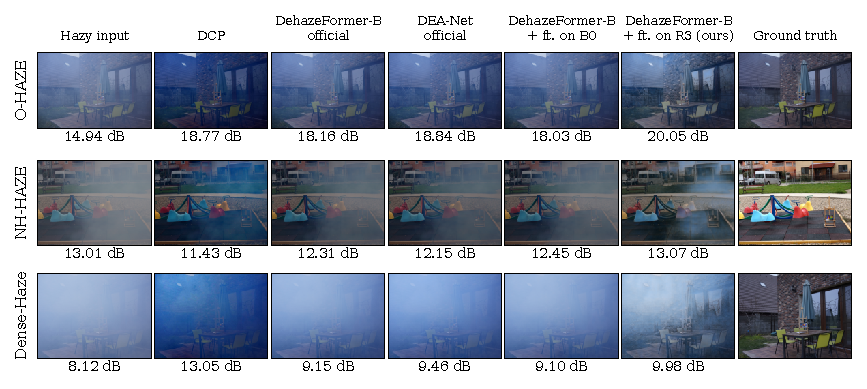
\includegraphics[width=\linewidth]{figs/qualitative.pdf}
\caption{Qualitative comparison (PSNR under each image). Columns five and six are the same published DehazeFormer-B checkpoint fine-tuned for the same number of steps on RESIDE's hazy images (B0) or on our haze (R3). Images were chosen by median improvement, not by best case.}
\label{fig:qual}
\end{figure}

% =====================================================================
\section{Conclusions}
\label{sec:conclusion}

We asked which parts of synthetic haze formation decide how well a dehazing network transfers to real haze, and answered it with a controlled study in which only one component changes between training sets. Four findings stand out in these preliminary runs. First, haze built on metric depth, with a realistic distribution of density and an airlight colour matched to the target data, improves clearly over RESIDE's synthesis of the same images: 1.0--1.4\,dB PSNR and 0.04--0.07 SSIM from scratch (three seeds), and up to 2.4\,dB when fine-tuning a published model. Second, the calibration matters more than we expected. Removing it removes the gain. Calibrating on a different real dataset keeps most of the structural (SSIM) gain but not the PSNR gain, which on these benchmarks largely reflects matching their colour cast. Third, compositing in linear radiance adds up to 0.9\,dB when training from scratch on target-calibrated haze, but not with RTTS calibration or when fine-tuning. Fourth, post-haze sensor noise and our spatially varying extinction reduce accuracy in this setting. Our initial hypothesis, that the camera model matters more than heterogeneity, is not supported: the camera model was close to neutral, and heterogeneity had the larger effect, in the harmful direction. A synthesis pipeline is therefore most useful when its haze statistics can be fitted to unlabelled images of the domain it will be used in, and metric depth is what makes those statistics controllable.

\paragraph{Limitations.} The schedules are short (about 56 epochs over 1{,}000 images), most arms have one seed, and the headline comparisons have two or three. Components were changed one at a time, not in a full factorial design, so interactions are not measured. The paired test sets use haze-machine haze and contain 155 images in total. The main comparisons use a calibration on the test sets' hazy inputs; the RTTS-calibrated controls show that the PSNR gain depends on it, and they have one seed each. RTTS detection was evaluated on a 500-image subset and did not separate methods. We did not compute LPIPS or FADE, and we did not evaluate driving datasets such as Foggy Zurich or ACDC.

\paragraph{Future work.} The most direct extension is to calibrate on unlabelled hazy images from a held-out part of each target domain, which removes the overlap with the test images, and to run the same study at full scale (all 3{,}000 images or more, full schedules, three seeds, a full factorial over the components that matter) and to test the resolution explanation for the noise result by matching noise to the test resolution. Beyond that, two directions follow from this work. The first is forward rendering of a calibrated participating medium into 3D Gaussian-splatting reconstructions of real scenes, which would replace monocular depth with true multi-view geometry while keeping real photographic content. The second is a wavelength-dependent extinction model for urban pollution haze, whose optical properties differ from the near-neutral fog in current benchmarks.

\bibliographystyle{plainnat}
\bibliography{refs}

\appendix
\section{Absolute results for all DehazeFormer-T arms}
\begin{table}[h]
\caption{DehazeFormer-T trained from scratch on each arm (mean over seeds). Best value per column in bold.}
\label{tab:arms}
\centering
\small
\resizebox{\linewidth}{!}{\begin{tabular}{llccccccc}
\toprule
Arm & Hazy-image formation & \multicolumn{2}{c}{O-HAZE} & \multicolumn{2}{c}{NH-HAZE} & \multicolumn{2}{c}{Dense-Haze} & Seeds \\
\cmidrule(lr){3-4}\cmidrule(lr){5-6}\cmidrule(lr){7-8}
 & & PSNR & SSIM & PSNR & SSIM & PSNR & SSIM & \\
\midrule
B0 & RESIDE-OTS hazy images (official synthesis) & 15.88 & 0.673 & 12.08 & 0.483 & 10.79 & 0.422 & 3 \\
N0 & sRGB ASM, grey airlight & 14.87 & 0.701 & 11.62 & 0.518 & 10.08 & 0.426 & 1 \\
R0\_uncal & sRGB ASM, no density calibration & 15.72 & 0.670 & 12.16 & 0.488 & 10.51 & 0.422 & 1 \\
R0\_rtts & sRGB ASM, calibrated on RTTS only & 15.79 & 0.730 & 12.27 & 0.550 & 11.25 & 0.443 & 1 \\
R0 & sRGB ASM, sky-coloured airlight & 17.25 & 0.743 & 13.10 & 0.556 & \textbf{12.12} & 0.459 & 3 \\
R1 & + linear-radiance compositing & \textbf{18.17} & \textbf{0.757} & \textbf{13.44} & \textbf{0.573} & 12.02 & 0.458 & 3 \\
R1\_rtts & R1, calibrated on RTTS only & 15.83 & 0.733 & 12.24 & 0.557 & 11.40 & 0.440 & 1 \\
R2 & + post-haze sensor noise & 17.35 & 0.737 & 13.09 & 0.551 & 11.53 & 0.460 & 1 \\
R3 & + randomised ISP + JPEG & 17.64 & 0.734 & 13.11 & 0.541 & 11.82 & \textbf{0.464} & 2 \\
R3N & R3 without sensor noise & 18.16 & 0.750 & 13.36 & 0.561 & 12.03 & 0.461 & 1 \\
H & R0 + heterogeneous extinction & 15.47 & 0.708 & 12.52 & 0.536 & 9.72 & 0.423 & 1 \\
R3H & R3 + heterogeneous extinction & 15.46 & 0.698 & 12.92 & 0.534 & 9.59 & 0.418 & 1 \\
\bottomrule
\end{tabular}}
\end{table}

\section{Implementation and reproducibility}
The full code (synthesis, training, evaluation, statistics and report tables) is organised as a single restart-safe pipeline. \texttt{haze/synth.py} implements the arms, \texttt{haze/isp.py} the camera model, \texttt{prepare\_depth.py} and \texttt{prepare\_params.py} the depth estimation and the stored visibility and airlight draws, \texttt{train.py} the shared training loop, and \texttt{eval\_paired.py} and \texttt{eval\_rtts.py} the evaluation. \texttt{stats.py} computes the bootstrap intervals. A five-to-eight-hour preliminary protocol (\texttt{quick.py}) measures each model's speed and divides the GPU budget across all runs, and produced every number in this report. Unit tests check, among other things, that all arms share their random draws, that the camera model is the identity when its random parameters are neutral, and that our SSIM matches the reference implementation.

\end{document}
